\documentclass[a4paper]{article}
\usepackage[english]{babel}
\usepackage[utf8]{inputenc}
\usepackage{fancyhdr}
\usepackage{hyperref}
\usepackage{amsmath,amsfonts,amssymb,amsthm}
\usepackage[a4paper, bottom=1.3in, top=1.3in, right=1in, left=1in]{geometry}
\usepackage[usenames,dvipsnames]{xcolor}
\usepackage[lined,boxed]{algorithm2e}
\usepackage{natbib}
\usepackage{dsfont}
\usepackage{tikz}
\usepackage{subcaption}
\usepackage{listings}
\usepackage{stmaryrd}
\usetikzlibrary{calc}
\definecolor{amaranth}{rgb}{0.9, 0.17, 0.31}
\newcommand{\rcol}[1]{{\color{amaranth}#1}}

\usepackage{todonotes}
\newcommand{\todomp}[1]{\todo[color=Green!10, inline]{\small MP: #1}}
\newcommand{\todompout}[1]{\todo[color=Green!10]{\scriptsize MP: #1}}

\newcommand{\wh}[1]{\widehat{#1}}
\newcommand{\wt}[1]{\widetilde{#1}}
\newcommand{\transp}{\intercal}

%%%%%%%%%%%%%%%%%%%%%%%%%%%%%%%%%%%%%%%%%%%
% Insert your name here
\newcommand{\fullname}{Raphael Reme}
%%%%%%%%%%%%%%%%%%%%%%%%%%%%%%%%%%%%%%%%%%%

\newcommand{\lecture}[3]{
   \pagestyle{myheadings}
   \thispagestyle{plain}
   \newpage
   \setcounter{page}{1}
   \noindent
   \begin{center}
   \framebox{
      \vbox{\vspace{2mm}
              \hbox to .97\textwidth { {\bf MVA: Reinforcement Learning (2020/2021) \hfill Homework 3} }
       \vspace{6mm}
       \hbox to .97\textwidth { {\Large \hfill #1 \hfill } }
       \vspace{6mm}
       \hbox to .97\textwidth { {Lecturers: \it A. Lazaric, M. Pirotta  \hfill {{\footnotesize(
           December 10, 2020
        %    \today
           )}}} }
      \vspace{2mm}}
   }
   \end{center}
   Solution by {\color{amaranth}\fullname}
   \markboth{#1}{#1}
   \vspace*{4mm}
}


\DeclareMathOperator*{\argmax}{\arg\,\max}
\DeclareMathOperator*{\argmin}{\arg\,\min}
\DeclareMathOperator*{\arginf}{\arg\,\inf}


\setlength{\parindent}{0cm}
\begin{document}
\lecture{Exploration in Reinforcement Learning (theory)}{3}


\pagestyle{fancy}
\fancyhf{}
\rhead{Full name: {\color{amaranth}\fullname}}
\lhead{Exploration in Reinforcement Learning}
\cfoot{\thepage}

\textbf{Instructions}
\begin{itemize}
    \item The deadline is \textbf{January 10, 2021. 23h00}
    \item By doing this homework you agree to the \emph{late day policy, collaboration and misconduct rules} reported on \href{https://piazza.com/class/kf86owfvi2u2lg?cid=8}{Piazza}.
    \item \textbf{Mysterious or unsupported answers will not receive full credit}.
          A correct answer, unsupported by calculations, explanation, or algebraic work will receive no credit; an incorrect answer supported by substantially correct calculations and explanations might still receive partial credit.
    \item Answers should be provided in \textbf{English}.
\end{itemize}


\section{UCB}
Denote by $S_{j,t} = \sum_{k=1}^t X_{i_k,k} \cdot \mathds{1}(i_k = a)$ and by $N_{j,t} = \sum_{k=1}^t \mathds{1}(i_k = j)$ the cumulative reward and number of pulls of arm $j$ at time $t$. Denote by $\wh\mu_{j,t} = \frac{S_{j,t}}{N_{j,t}}$ the estimated mean. Recall that, at each timestep $t$, UCB plays the arm $i_t$ such that
\[
    i_t \in \argmax_{j} \wh\mu_{j,t} + U(N_{j,t}, \delta)
\]
Is $\wh\mu_{j,t}$ an unbiased estimator (i.e., $\mathbb{E}_{UCB}[\wh\mu_{j,t}] = \mu_j$)? Justify your answer.

\subsection*{Answer}
The first intuition could be that it's independent of $N_{j,t}$ and that we could consider that
$\forall n, \mathbb{E}[\wh\mu_{j,t}|N_{j,t}=n] = \mathbb{E}[\frac{S_{j,t}}{N_{j,t}}| N_{j,t}=n]
    = \frac{1}{n}\mathbb{E}[\sum_k X_{j,k} \mathds{1}(i_k = j) | N_{j,t}=n] = \frac{n}{n}\mathbb{E}[X_{j, 0}] = \mu_j$. And we could be tempted to conclude that
therefore it's unbiased. But I will try to show that it's much more complicated. Indeed the information $N_{j, t} = n$ is not innocent at all. And the
intuition that we should rather have, is that we resample more if we have high values of previous $(X_{j, k})_k$.

Let's focus with $A$ actions = $\llbracket 1, A\rrbracket$ and assume that that $U(0, \delta) = \infty$. Then the first $A$ steps of the algorithm will
choose all the actions once by definition of $i_t$. (Note that for $t < A$ then $\exists j, N_{j, t} = 0$ and then $\wh\mu_{j, t}$ is not well defined).
The definition of $i$ is also not very clear. I will assume that $i_1 = 1$ and that
$i_{t+1} \in \text{argmax}_{j \in [1, A]}\, \wh\mu_{j,t} + U(N_{j,t}, \delta)$. (Otherwise $i_t$ would depend on informations we don't have at the moment!)

Let's consider $t = A$. We have $\forall j, N_{j, t} = 1$. (The order of the $i_k$ is irrelevant and I will suppose them ordered:
$\forall k \in [1, A], i_k = k$). Then $i_{t+1} \in \text{argmax}_{j \in [1, A]}\, \wh\mu_{j,t} + U(N_{j,t}, \delta) = \text{argmax}_{j \in [1, A]} X_{j, j}$.

This shows that we sample the action $t = A + 1$ according to the best rewards we got. And this could lead to negative bias: indeed
if we get a low value for an action (lower than the expectation for instance), we will less resample it than if we had got a high value
for this action. Low values of the laws of our rewards are over represented in our empirical mean.
\vspace{8px}\\
Example: Let's use $A = 2, t = 3$ and $X_{1, k} \sim 2\mathbb{B}(p) + 1$, $X_{2, k} \sim 2\mathbb{B}(q)$. We have
$\mathbb{P}(X_{1, k} = 3) = p, \mathbb{P}(X_{1, k} = 1) = 1-p, \mathbb{P}(X_{2, k} = 2) = q, \mathbb{P}(X_{2, k} = 0) = 1-q$.
And $\mu_1 = 2p + 1, \mu_2 = 2q$. Now we can see that $\wh\mu_{1, 3} = X_{1, 1} + \frac{1}{2}\mathds{1}_{i_3 = 1}(X_{1, 3} - X_{1, 1})$.

Then $\mathbb{E}[\wh\mu_{1, 3}] = \mu_1 + \frac{1}{2}\mathbb{E}[\mathds{1}_{i_3 = 1}(X_{1, 3} - X_{1, 1})]$. And as $(i_3 = 1) = (X_{1,1} = 3)\bigcup(X_{1, 1} = 1)\cap(X_{2,2} = 0)$:
\begin{equation*}
    \begin{aligned}
        \mathbb{E}[\mathds{1}_{i_3 = 1}(X_{1, 3} - X_{1, 1})] & = \sum_{\substack{x_1 \in \{1, 3\}                      \\ x_2 \in \{0, 2\} \\ x_3 \in \{1, 3\}}} \mathbb{P}(X_{1, 1} = x_1)
        \mathbb{P}(X_{2, 2} = x_2)\mathbb{P}(X_{1, 3} = x_3)\mathds{1}_{i_3 = 3}(x_3 - x_1)                             \\
                                                              & = \sum_{\substack{x_1 \in \{1, 3\}                      \\ x_2 \in \{0, 2\} \\ x_3 \in \{1, 3\}}} p_1(x_1)
        p_2(x_2) p_1(x_3)(\mathds{1}_{x_1 = 3} + \mathds{1}_{x_1 = 1}\mathds{1}_{x_2 = 0})(x_3 - x_1)                   \\
                                                              & = p \sum_{\substack{x_2 \in \{0, 2\}                    \\ x_3 \in \{1, 3\}}} p_2(x_2)p_1(x_3) (x_3 - 3) +  (1-p)(1-q) \sum_{x_3 \in \{1, 3\}} p_1(x_3) (x_3 - 1)\\
                                                              & = p \times 1 \times (\mu_1 - 3) + (1-p)(1-q)(\mu_1 - 1) \\
                                                              & = p(2p - 2) - (1-p)(1-q)(2p)                            \\
                                                              & = -2p(1-p)q                                             \\
                                                              & < 0
    \end{aligned}
\end{equation*}

Hence $\boxed{\mathbb{E}[\wh\mu_{1, 3}] < \mu_1}$. (This also holds for $\mu_2$) In this example we have a negative bias.
This shows that it can't be an unbiased estimator in the general case .

\section{Best Arm Identification}
In best arm identification (BAI), the goal is to identify the best arm in as few samples as possible.
We will focus on the fixed-confidence setting where the goal is to identify the best arm with high probability $1-\delta$ in as few samples as possible.
A player is given $k$ arms with expected reward $\mu_i$. At each timestep $t$, the player selects an arm to pull ($I_t$), and they observe some reward ($X_{I_t,t}$) for that sample.
At any timestep, once the player is confident that they have identified the best arm, they may decide to stop.

\paragraph{$\delta$-correctness and fixed-confidence objective.}
Denote by $\tau_\delta$ the stopping time associated to the stopping rule, by $i^\star$ the best arm and by $\wh{i}$ an estimate of the best arm.
An algorithm is $\delta$-correct if it predicts the correct answer with probability at least $1-\delta$. Formally, if $\mathbb{P}_{\mu_1, \ldots, \mu_k}(\wh{i} \neq i^\star) \leq \delta$ and $\tau_{\delta} < \infty$ almost surely for any $\mu_1, \ldots, \mu_k$.
Our goal is to find a $\delta$-correct algorithm that minimizes the sample complexity, that is, $\mathbb{E}[\tau_\delta]$ the expected number of sample needed to predict an answer.

\vspace{.2in}
\underline{Notation}
\begin{itemize}
    \item $I_t$: the arm chosen at round $t$.
    \item $X_{i,t} \in [0,1]$: reward observed for arm $i$ at round $t$.
    \item $\mu_i$: the expected reward of arm $i$.
    \item $\mu^\star = \max_i \mu_i$.
    \item $\Delta_i = \mu^\star - \mu_i$: suboptimality gap.
\end{itemize}

Consider the following algorithm
\begin{algorithm}[h]
    \SetAlgoLined
    \DontPrintSemicolon
    \KwIn{$k$ arms, confidence $\delta$}
    $S = \{1, \ldots, k\}$\;
    \For{$t = 1, \ldots$}{
        Pull \textbf{all} arms in $S$\;
        $S = S \setminus \Big\{i \in S \;:\; \exists j \in S,\; \wh{\mu}_{j,t} - U(t,\delta) \geq \wh{\mu}_{i,t} + U(t, \delta)  \Big\}$\;
        \If{$|S|=1$}{
            STOP\;
            \textbf{return} $S$\;
        }
    }
\end{algorithm}

The algorithm maintains an active set $S$ and an estimate of the empirical reward of each arm $\wh\mu_{i,t} = \frac{1}{t} \sum_{j=1}^t X_{i,j}$.
\begin{itemize}
    \item Compute the function $U(t,\delta)$ that satisfy the any-time confidence bound. For any arm $i \in [k]$
          \[
              \mathbb{P}\left(\bigcup_{t=1}^{\infty} \left\{ | \wh{\mu}_{i,t} - \mu_i | > U(t,\delta)\right\} \right) \leq \delta
          \]
          Use Hoeffding's inequality.
    \item Let $\mathcal{E} = \bigcup_{i=1}^{k}\bigcup_{t=1}^{\infty} \left\{ | \wh{\mu}_{i,t} - \mu_i | > U(t,\delta')\right\}$. Using previous result shows that $\mathbb{P}(\mathcal{E}) \leq \delta$ for a particular choice of $\delta'$. This is called ``bad event'' since it means that the confidence intervals do not hold.
    \item Show that with probability at least $1-\delta$, the optimal arm $i^\star =\argmax_i \{\mu_{i}\}$ remains in the active set $S$. Use your definition of $\delta'$ and start from the condition for arm elimination. From this, use the definition of $\neg \mathcal{E}$.
    \item Under event $\neg \mathcal{E}$, show that an arm $i \neq i^\star$ will be removed from the active set when $\Delta_i \geq C_1 U(t, \delta')$ where $C_1 > 1$ is a constant. Compute the time required to have such condition for each non-optimal arm. Use the condition of arm elimination applied to arm $i^\star$.
    \item Compute a bound on the sample complexity (after how many rounds the algorithm stops) for identifying the optimal arm w.p. $1-\delta$.
\end{itemize}

Note that also a variations of UCB are effective in pure exploration.

\subsection*{Answers}
\subsubsection*{1-}

First the Hoeffding's inequality can be stated as
$\forall \delta, t, i, \; \mathbb{P}\left(|\wh{\mu}_{i,t} - \mu_i| > \sqrt{\frac{\log\frac{2}{\delta}}{2t}}\right) \le \delta$.

Now let's define $\forall t \ge 1, B_t = \{| \wh{\mu}_{i,t} - \mu_i | > U(t,\delta) |\}$, $\forall n \ge 1, A_n = \bigcup_{t=1}^n B_t$. We are trying
to find $U(t, \delta)$ such that $\mathbb{P}\left(\bigcup_{t=1}^{\infty} B_t \right) \leq \delta$.

With our notations we have $A_n \subset A_{n + 1}$ and therefore
\begin{equation*}
    \begin{aligned}
        \mathbb{P}\left(\bigcup_{t=1}^{\infty} B_t \right) & = \mathbb{P}\left(\bigcup_{t=1}^{\infty} A_n \right)      \\
                                                           & = \lim_{n \rightarrow \infty} \mathbb{P}\left(A_n \right)
    \end{aligned}
\end{equation*}

Moreover $\mathbb{P}\left(A_n\right) = \mathbb{P}\left(\bigcup_{t=1}^{n} B_t \right) \le \sum_{t=1}^n \mathbb{P}\left( B_t \right) \le \sum_{t=1}^\infty \mathbb{P}\left( B_t \right) $.

Let's define $U(t, \delta) = \sqrt{\frac{\log\frac{2}{\frac{1}{2^t}\delta}}{2t}} = \sqrt{\frac{\log\frac{2^{t+1}}{\delta}}{2t}}$
then the Hoeffding's inequality applied to $B_t$ gives

\begin{equation*}
    \begin{aligned}
        \mathbb{P}\left(B_t\right) & = \mathbb{P}\left(|\wh{\mu}_{i,t} - \mu_i| > U(t, \delta)\right) \\
                                   & \le \frac{1}{2^t}\delta
    \end{aligned}
\end{equation*}

Thus we have $\forall n \ge 1$:
\begin{equation*}
    \begin{aligned}
         & \mathbb{P}\left(A_n\right) \le \sum_{t=1}^\infty \mathbb{P}\left( B_t \right)                                                                                                                           \\
         & \mathbb{P}\left(A_n\right) \le \sum_{t=1}^\infty \frac{1}{2^t}\delta                                                                                                                                    \\
         & \mathbb{P}\left(A_n\right) \le \delta                                                                                                                                                                   \\
         & \lim_{n\leftarrow\infty}\mathbb{P}\left(A_n\right) \le \delta                                                                                                                                           \\
         & \mathbb{P}\left(\bigcup_{t=1}^{\infty} B_t \right) \le \delta                                                                                                                                           \\
         & \mathbb{P}\left(\bigcup_{t=1}^{\infty} \left\{ | \wh{\mu}_{i,t} - \mu_i | > U(t,\delta)\right\} \right)  \leq \delta & \text{with } \boxed{U(t, \delta) = \sqrt{\frac{\log\frac{2^{t+1}}{\delta}}{2t}}} \\
    \end{aligned}
\end{equation*}


\paragraph*{Correction after Q4:}
This choice of $U$ is valid but not good enough because here $U$ doesn't converge to 0 when $t$ goes to infinity (in this case it converges to
$\sqrt{\frac{\log2}{2}}$).


We have to choose U such that
$\sum_{t=1}^\infty \mathbb{P}(B_t) = \delta$ and so that U converges to 0. As we have seen the choice of $\mathbb{P}(B_t)$ gives U.
And an exponential choice in t leads to a function $U$ that doesn't converge towards 0. It seems obvious that a polynomial one would be good.
($\mathbb{P}(B_t) \propto \frac{1}{t^n}$). Let's prove it! (I will choose $n=2$ here)

Let's defined $C = \sum_{t=1}^\infty \frac{1}{t^2} = \frac{\pi^2}{6}$. And with the Hoeffding's inequality let's choose $U$ such that
$\mathbb{P}(B_t) = \frac{\delta}{Ct^2}$:
$U(t, \delta) = \sqrt{\frac{\log\frac{2Ct^2}{\delta}}{2t}} =  \sqrt{\frac{2\log t + \log\frac{2C}{\delta}}{2t}}$.

With this $U$ we have $\forall \delta, \lim_{t\rightarrow\infty} U(t, \delta) = 0$ and $\sum_{t=1}^{\infty} \mathbb{P}(B_t) = \delta$.

Therefore we have:
\begin{equation*}
    \begin{aligned}
        \mathbb{P}\left(\bigcup_{t=1}^{\infty} \left\{ | \wh{\mu}_{i,t} - \mu_i | > U(t,\delta)\right\} \right)  \leq \delta &  & \text{with } \boxed{U(t, \delta) = \sqrt{\frac{\log\frac{2Ct^2}{\delta}}{2t}}} \\
    \end{aligned}
\end{equation*}

\subsubsection*{2-}
With $C_i = \bigcup_{t=1}^{\infty} \left\{ | \wh{\mu}_{i,t} - \mu_i | > U(t,\delta')\right\}$, we have:
\begin{equation*}
    \begin{aligned}
        \mathbb{P}\left(\bigcup_{i=1}^{k}C_i\right) & \le \sum_{i=1}^k \mathbb{P}\left( C_i \right)                                                         \\
                                                    & \le k\delta'                                  &  & \text{(As $\forall i, \mathbb{P}(C_i) < \delta'$)} \\
    \end{aligned}
\end{equation*}

Therefore with $\boxed{\delta' = \frac{\delta}{k}}$, then $\mathbb{P}(\mathcal{E}) < \delta$.

\subsubsection*{3-}
We have shown that $\mathbb{P}(\mathcal{E}) < \delta$. Therefore we have $\mathbb{P}(\neg \mathcal{E}) = 1 - \mathbb{P}(\mathcal{E}) > 1 - \delta$.

Now let's denote by $A$ the event stating that the optimal arm remains in S:
\begin{equation*}
    A = \bigcap_{t=1}^\infty\left\{i^\star \notin \Big\{i \in S \;:\; \exists j \in S,\; \wh{\mu}_{j,t} - U(t,\delta') \geq \wh{\mu}_{i,t} + U(t, \delta')  \Big\}\right\}
\end{equation*}
(Note: I'm using $\delta'$ as input of the algorithm rather than $\delta$ otherwise it won't work. And I will assume that $i^\star$ is unique. If
it exists $j^\star$ s.t. $mu_{j^\star} = \mu^\star$, we could have a case were $i^\star$ is removed. But $j^\star$ would stay.)

I will show that $\neg \mathcal{E} \subset A$: if $\neg \mathcal{E}$ occurs then so does $A$.

Assuming that $\neg \mathcal{E}$ has happened. Then $\forall i, t, |\wh{\mu}_{i,t} - \mu_i | < U(t,\delta')$.
Let $t \ge 1$, $j\in S\setminus\{i^\star\}$, we have :
\begin{equation*}
    \begin{aligned}
        |\wh{\mu}_{j,t} - \mu_j | \le U(t,\delta') &  & \text{and} &  & |\wh{\mu}_{i^\star,t} - \mu^\star | \le U(t,\delta')                                   \\
        \wh{\mu}_{j,t} - \mu_j  \le U(t,\delta')   &  & \text{and} &  & \mu^\star - \wh{\mu}_{i^\star,t} \le U(t,\delta')    &  & \text{(As  $\pm x \le |x|$)} \\
    \end{aligned}
\end{equation*}

Then we have:
\begin{equation*}
    \begin{aligned}
        \wh{\mu}_{j,t} - \mu_j + \mu^\star - \wh{\mu}_{i^\star,t} \le 2U(t,\delta')                              \\
        \wh{\mu}_{j,t} - \mu_j + \mu^\star - \wh{\mu}_{i^\star,t} < 2U(t,\delta') + \Delta_j &  & (\Delta_j < 0) \\
        \wh{\mu}_{j,t} - \mu_j + \mu^\star - \wh{\mu}_{i^\star,t} < 2U(t,\delta') + \mu^\star - \mu_j            \\
        \wh{\mu}_{j,t} - \wh{\mu}_{i^\star,t} < 2U(t,\delta')                                                    \\
        \wh{\mu}_{j,t} - U(t,\delta') < \wh{\mu}_{i^\star,t} + U(t,\delta')                                      \\
    \end{aligned}
\end{equation*}

And as $U(t, \delta') > 0$ we also have this inequality for $j = i^\star$. Therefore
$\forall t \ge 1, i^\star \notin \Big\{i \in S \;:\; \exists j \in S,\; \wh{\mu}_{j,t} - U(t,\delta') \geq \wh{\mu}_{i,t} + U(t, \delta')  \Big\}$.
And thus we are in A.

We've shown that $\neg\mathcal{E} \subset A $ (any $w$ realising $\neg\mathcal{E}$ will also realised $A$) and therefore
$\boxed{\mathbb{P}(A) \ge \mathbb{P}(\neg \mathcal{E}) \ge 1 - \delta}$, that is to say that the optimal arm remains in $S$ with probability at least
$1 - \delta$.

\subsubsection*{4-}

Let's call $D(S) = \Big\{i \in S \;:\; \exists j \in S,\; \wh{\mu}_{j,t} - U(t,\delta') \geq \wh{\mu}_{i,t} + U(t, \delta')  \Big\}$. (Note that
$S$ depends on $t$)

Let $i \neq i^\star$ we want to show that $\exists t \ge 1$ such that $i \in D(S)$ and find this $t$.

Now as in the previous question, let's assume that $\neg \mathcal{E}$ has happened. Then we've shown that $\forall t \ge 1, i^\star \in S$. And we will use
that knowledge to show that $\wh{\mu}_{i^\star,t} - U(t,\delta') \geq \wh{\mu}_{i,t} + U(t, \delta')$ under a condition on $t$.
(And thus for that $t, i \in D(S)$ and is removed from the active set.)

As before we have:
\begin{equation*}
    \begin{aligned}
        \wh{\mu}_{i,t} - \mu_i + \mu^\star - \wh{\mu}_{i^\star,t} & \le 2U(t,\delta')                                                                                               \\
        \wh{\mu}_{i,t} + \Delta_i - \wh{\mu}_{i^\star,t}          & \le 2U(t,\delta')                                                                                               \\
        \wh{\mu}_{i^\star,t}                                      & \ge \wh{\mu}_{i,t} - 2U(t, \delta') + \Delta_i                                                                  \\
        \wh{\mu}_{i^\star,t} - U(t, \delta')                      & \ge \wh{\mu}_{i,t} + U(t, \delta') - 4U(t, \delta') + \Delta_i                                                  \\
        \wh{\mu}_{i^\star,t} - U(t, \delta')                      & \ge \wh{\mu}_{i,t} + U(t, \delta')                             & \text{If } \boxed{\Delta_i \ge 4U(t, \delta')} \\
    \end{aligned}
\end{equation*}

Therefore $\boxed{C_1 = 4}$.

Asusming that $i^\star$ is unique then, $\Delta_i > 0$ and as $\lim_{t\rightarrow\infty} U(t, \delta') = 0$ from Q1 (after correction):

\begin{equation*}
    \boxed{\exists t_i\ge 1,\, C_1U(t_i, \delta') \ge \Delta_i}
\end{equation*}
Let's fix $t_i = \inf_t \{t \ge 1, C_1U(t, \delta') \ge \Delta_i\}$. Then the sub-optimal arm $i$ is removed after at most $\lceil t_i \rceil$ iterations.

Let's try to express this $t_i$ w.r.t. $\Delta_i$ and $\delta$:
\begin{equation*}
    \begin{aligned}
        4U(t_i, \delta) \le \Delta_i                                                                                            \\
        \sqrt{\frac{\log\frac{\pi^2t_i^2}{3\delta}}{2t_i}} \le \frac{\Delta_i}{4}                                               \\
        \frac{\log\frac{\pi^2t_i^2}{3\delta}}{2t_i} \le \left(\frac{\Delta_i}{4}\right)^2                                       \\
        \frac{\log t_i}{t_i} + \frac{\log\frac{\pi^2}{3\delta}}{2t} \le \left(\frac{\Delta_i}{4}\right)^2                       \\
        \log{t_i} + A \le Bt_i &  & \text{With } A = \frac{\log\frac{\pi^2}{3\delta}}{2}, B = \left(\frac{\Delta_i}{4}\right)^2 \\
        Bt_i - \log t_i - A \ge 0                                                                                               \\
    \end{aligned}
\end{equation*}

Let's analyse this function $f(t) = Bt - \log t - A$. First as $\Delta_i \in ]0, 1]$, we have $0 < B \le \frac{1}{16}$. And I will suppose than $\delta < \frac{1}{3}$
(High values for $\delta$ have no interest and this will help to characterize $t_i$) then, $A > \log\pi > 1 > B$.

We can compute the derivative of $f: f'(t) = B - \frac{1}{t}$. $f'(t) = 0 \Leftrightarrow t = \frac{1}{B}$. As $f$ is convexe $f$ reaches a minimum
at $t=\frac{1}{B}$. And $f(1) = B - A < 0$. Therefore $f$ is negative on $[1, \frac{1}{B}]$ ($\frac{1}{B} > 1$).
And $f(t) \longrightarrow_{t \rightarrow \infty} \infty$.

Therefore there is a unique $t_0 \in [\frac{1}{B}, +\infty]$ such that $f(t_0) = 0$. And by definition of $t_i$ we have $t_i = t_0$
(because $t_0$ is the first $t \ge 1$ such that $f(t) \ge 0$). We thus have a first bound for $t_i$:

\begin{equation*}
    \begin{aligned}
        t_i & \ge \frac{1}{B}                       \\
            & \ge \left(\frac{4}{\Delta_i}\right)^2
    \end{aligned}
\end{equation*}

It's not an upperbound and therefore we can't deduce anything for the time needed to eliminate the sub-optimal arm $i$ from this equation (but still
it gives informations on $t_i$)

As $\log$ is concave it's below any of its tangent. I will use this to find an upperbound:

\begin{equation*}
    \begin{aligned}
        \forall x_0 > 0, t > 0,\; & \log(t) \le \log(x_0) + \frac{1}{x_0}(t - x_0)      \\
                                  & - \log(t) \ge -\frac{t}{x_0} + 1 - \log(x_0)        \\
                                  & f(t) \ge (B - \frac{1}{x_0})t + 1 - A - \log{x_0}   \\
                                  & f(t) \ge \frac{Bx_0 - 1}{x_0} t + 1 - A - \log{x_0} \\
    \end{aligned}
\end{equation*}

Let's use $x_0 = \frac{A}{B}$ (in order to use the fact that $A > 1$)
\begin{equation*}
    \begin{aligned}
        f(t) & \ge B\frac{A - 1}{A}t + 1 - A - \log A + \log B \\
    \end{aligned}
\end{equation*}

Now as $A > 1$ we have:
\begin{equation*}
    \begin{aligned}
        \forall t \ge A\frac{A - 1 + \log A - \log B}{B(A -1)},\; & B\frac{A - 1}{A}t + 1 - A - \log A + \log B \ge 0 \\
                                                                  & f(t) \ge 0                                        \\
    \end{aligned}
\end{equation*}

(If we don't assume that $\delta < \frac{1}{3}$ then we could still prove that $A > 0.5$ and use directly $x_0 = 2\frac{A}{B}$,
which leads to a similar results)

We have therefore $t_i \le A\frac{A - 1 + \log A - \log B}{B(A -1)}$ (as $t_i$ is the smallest $t$ that verify this equation.)

Assuming that $\delta$ (and $\Delta_i$) are small enough we can simplify the expression keeping only dominant terms:
\begin{equation*}
    A\frac{A - 1 + \log A - \log B}{B(A - 1)} + 1 \sim  16\frac{\log\frac{1}{\delta} - 2\log\Delta_i}{\Delta_i^2}
\end{equation*}

Finally $\boxed{t_i \le \alpha \frac{\log\frac{1}{\delta} - 2\log\Delta_i}{\Delta_i^2}}$ (With $\alpha$ a constante).

\subsubsection*{5-}

Finally if $i^\star$ is unique, then the algortihm will remove all sub-optimal arms $i \neq i^\star$ in at most
$T = \max_{i \neq i^\star} \lceil t_i \rceil$ iterations!

Let's define $\Delta = \min_{i \neq i^\star} \Delta_i$. From the previous question we have:

\begin{equation*}
    \begin{aligned}
        \forall i \neq i^\star,\; & t_i \le \alpha \frac{\log\frac{1}{\delta} - 2\log\Delta_i}{\Delta_i^2} \le \alpha \frac{\log\frac{1}{\delta} - 2\log\Delta}{\Delta^2} \\
                                  & \boxed{T \le \alpha \frac{\log\frac{1}{\delta} - 2\log\Delta}{\Delta^2}}
    \end{aligned}
\end{equation*}


\section{Bernoulli Bandits}
In this exercise, you compare KL-UCB and UCB empirically with Bernoulli rewards $X_t \sim Bern(\mu_{I_t})$.

\begin{itemize}
    \item Implement KL-UCB and UCB
          \begin{description}
              \item[KL-UCB:]
                    \[
                        I_t = \argmax_i \max \bigg\{ \mu \in [0,1] : d(\wh\mu_{i, t},\mu) \leq \frac{\log(1+t\log^2(t))}{N_{i,t}} \bigg\}
                    \]
                    where $d$ is the Kullback–Leibler divergence (see closed form for Bernoulli). A way of computing the inner $\max$ is through bisection (finding the zero of a function).
              \item[UCB:]
                    \[
                        I_t = \argmax_i \wh\mu_{i,t} + \sqrt{\frac{\log(1+t\log^2(t))}{2N_{i,t}}}
                    \]
                    that has been tuned for 1/2-subgaussian problems.
          \end{description}
    \item Let $n = 10000$ and $k = 2$. Plot the \underline{expected} regret of each algorithm as a function of $\Delta$ when $\mu_1 = 1/2$ and $\mu_2 = 1/2 + \Delta$.
    \item Repeat the above experiment with $\mu_1 = 1/10$ and $\mu_1 = 9/10$.
    \item Discuss your results.
\end{itemize}

\subsection*{Answers-}

\begin{figure}[h!]
    \centering
    \begin{subfigure}[b]{0.3\linewidth}
        
\includegraphics[width=\linewidth]{images/05}
    \end{subfigure}
    \begin{subfigure}[b]{0.3\linewidth}
        
\includegraphics[width=\linewidth]{images/01}
    \end{subfigure}
    \begin{subfigure}[b]{0.3\linewidth}
        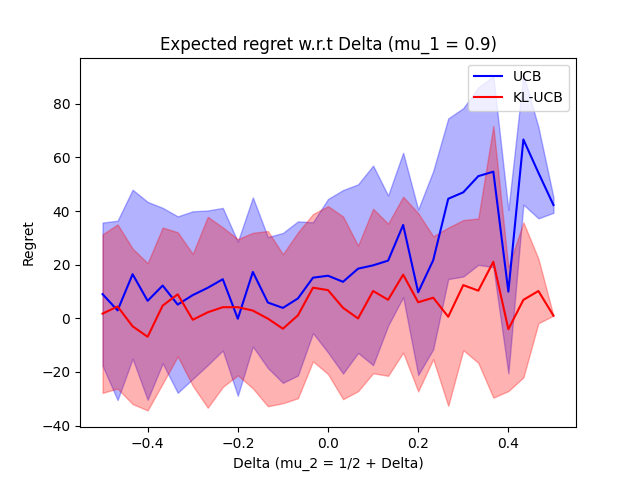
\includegraphics[width=\linewidth]{images/09}
    \end{subfigure}
    \caption{Expected regret for different $\mu_1$ (0.5, 0.1, 0.9)}
    \label{fig:results3}
\end{figure}

Those results have been obtained with 30 randoms runs of the algorithms. In order to reproduce them, you can run the code provided with:
\begin{lstlisting}{bash}
    $ python exercise3.py
    $ python exercise3.py --mu-1 0.1
    $ python exercise3.py --mu-1 0.9
\end{lstlisting}

It seems that even with 30 runs there are lots of uncertainty over our results and it's hard to conclude.

But the KL-UCB method seems to slightly outperform the UCB method, specially when $\mu_1$ is closed to $\mu_2$.

\section{Regret Minimization in RL}
Consider a finite-horizon MDP $M^\star = (S, A, p_h, r_h)$ with stage-dependent transitions and rewards. Assume rewards are bounded in $[0,1]$.
We want to prove a regret upper-bound for UCBVI. We will aim for the suboptimal regret bound ($T=KH$)
\[
    R(T) = \sum_{k=1}^K V^\star_1(s_{1,k}) - V^{\pi_k}_1(s_{1,k}) = \wt{O}(H^2S\sqrt{AK})
\]
Define the set of plausible MDPs as
\[
    \mathcal{M}_k = \{ M = (S,A, p_{h,k}, r_{h,k}) ~:~ r_{h,k}(s,a) \in \beta^r_{h,k}(s,a), p_{h,k}(\cdot|s,a) \in \beta^p_{h,k}(s,a)  \}
\]
Confidence intervals can be anytime or not.

\begin{itemize}
    \item Define the event $\mathcal{E} = \{\forall k, M^\star \in \mathcal{M}_k\}$. Prove that $\mathbb{P}(\neg\mathcal{E}) \leq \delta/2$. First step, construct a confidence interval for rewards and transitions for each $(s,a)$ using Hoeffding and Weissmain inequality (see appendix), respectively. So, we want that
          \[
              \mathbb{P}\Big(\forall k,h,s,a : |r_{hk}(s,a) - r_h(s,a)| \leq \beta_{hk}^r(s,a) \wedge \|\wh{p}_{hk}(\cdot|s,a) - p_{h}(\cdot|s,a)\|_1\leq \beta_{hk}^p(s,a)\Big) \geq 1-\delta/2
          \]

    \item Define the bonus function and consider the Q-function computed at episode $k$
          \[
              Q_{h,k}(s,a) = \wh{r}_{h,k}(s,a) + b_{h,k}(s,a) + \sum_{s'} \wh{p}_{h,k}(s'|s,a) V_{h+1,k}(s')
          \]
          with $V_{h,k}(s) = \min\{H, \max_a Q_{h,k}(s,a)\}$. Recall that $V_{H+1,k}(s) = V_{H+1}^\star(s) = 0$.
          Prove that under event $\mathcal{E}$, $Q_k$ is optimistic, i.e.,
          \[
              Q_{h,k}(s,a) \geq Q^{\star}_h(s,a), \forall s,a
          \]
          where $Q^\star$ is the optimal Q-function of the unknown MDP $M^\star$.
          Note that $\wh{r}_{H,k}(s,a) + b_{h,k}(s,a) \geq r_{h,k}(s,a)$ and thus $Q_{H,k}(s,a) \geq Q^\star_H(s,a)$ (for a properly defined bonus). Then use induction to prove that this holds for all the stages $h$.

    \item In class we have seen that
          \begin{equation}
              \label{eq:ucbvi_rec}
              \delta_{hk}(s_{1,k}) \leq \sum_{h=1}^H Q_{hk}(s_{hk},a_{hk}) - r(s_{hk},a_{hk}) - \mathbb{E}_{Y\sim p(\cdot|s_{hk},a_{hk})}[V_{h+1,k}(Y)]) + m_{hk}
          \end{equation}
          where $\delta_{hk}(s)=V_{hk}(s) - V_h^{\pi_k}(s)$ and $m_{hk} = \mathbb{E}_{Y\sim p(\cdot|s_{hk},a_{hk})}[\delta_{h+1,k}(Y)] - \delta_{h+1,k}(s_{h+1,k})$.
          We now want to prove this result. Denote by $a_{hk}$ the action played by the algorithm (you will have to use the greedy property).
          \begin{enumerate}
              \item Show that $V^{\pi_{k}}_h(s_{hk}) = r(s_{hk},a_{hk}) + \mathbb{E}_{p}[V_{h+1,k}(s')] - \delta_{h+1,k}(s_{h+1,k}) - m_{h,k}$
              \item Show that $V_{h,k}(s_{hk}) \leq Q_{h,k}(s_{hk},a_{hk})$.
              \item Putting everything together prove Eq.~\ref{eq:ucbvi_rec}.
          \end{enumerate}

    \item Since $(m_{hk})_{hk}$ is an MDS, using Azuma-Hoeffding we show that with probability at least $1-\delta/2$
          \[
              \sum_{k,h} m_{hk} \leq 2H\sqrt{KH \log(2/\delta)}
          \]
          Show that the regret is upper bounded with probability $1-\delta$ by
          \[
              R(T) \leq \sum_{kh} b_{hk}(s_{hk},a_{hk}) + 2H\sqrt{KH \log(2/\delta)}
          \]

    \item Finally, we have that
          \begin{align*}
              \sum_{h,k} \frac{1}{\sqrt{N_{hk}(s_{hk},a_{hk})}} = \sum_{h=1}^H\sum_{s,a} \sum_{i=1}^{N_{h,K}(s,a)} \frac{1}{\sqrt{i}} \leq \sum_{h=1}^H\sum_{s,a} \sqrt{N_{hK}(s,a)}
          \end{align*}
          Complete this by showing an upper-bound of $H\sqrt{SAK}$, which leads to $R(T) \lesssim H^2S\sqrt{AK}$
\end{itemize}

\begin{algorithm}[t]
    \DontPrintSemicolon
    Initialize $Q_{h1}(s,a) = 0$ for all $(s,a) \in S\times A$ and $h=1,\ldots,H$
    \vspace{0.1in}

    \For{$k=1, \ldots, K$}{
    Observe initial state $s_{1k}$ \textit{(arbitrary)}

    Estimate empirical MDP $\wh{M}_k = (S, A, \wh{p}_{hk}, \wh{r}_{hk}, H)$ from $\mathcal{D}_{k}$
    {\scriptsize
            \begin{align*}
                \wh{p}_{hk}(s'|s,a) = \frac{\sum_{i=1}^{k-1} \mathds{1}\{(s_{hi},a_{hi},s_{h+1,i})=(s,a,s')\}}{N_{hk}(s,a)} , \quad
                \wh{r}_{hk}(s,a)    = \frac{\sum_{i=1}^{k-1} r_{hi} \cdot \mathds{1}\{(s_{hi},a_{hi})=(s,a)\}}{N_{hk}(s,a)}
            \end{align*}
        }

    Planning (by backward induction) for $\pi_{hk}$ using $\wh{M}_k$\;
    \For{$h=H,\ldots,1$}{
        $Q_{h,k}(s,a) = \wh{r}_{h,k}(s,a) + b_{h,k}(s,a) + \sum_{s'} \wh{p}_{h,k}(s'|s,a) V_{h+1,k}(s')$\;
        $V_{h,k}(s) = \min\{H, \max_a Q_{h,k}(s,a)\}$\;
    }
    Define $\pi_{h,k}(s) = \argmax_{a} Q_{h,k}(s,a)$, $\forall s,h$\;

    \For{$h=1, \ldots, H$}{
    Execute $a_{hk} = \pi_{hk}(s_{hk})$\;
    Observe $r_{hk}$ and $s_{h+1,k}$\;
    $N_{h,k+1}(s_{hk},a_{hk}) = N_{h,k}(s_{hk},a_{hk}) + 1$
    }
    }
    \caption{UCBVI}
    \label{alg:ucbvi}
\end{algorithm}

\subsection*{Answers}
\subsubsection*{1-}
\begin{equation*}
    \begin{aligned}
        \neg \mathcal{E} & = \bigcup_{k=1}^K \{M^\star \notin M_k\}                                                                                                                                \\
                         & = \bigcup_{k=1}^K \bigcup_{s \in S} \bigcup_{a\in A} \bigcup_{h=1}^H \{r_{h, k}(s ,a) \notin B^r_{h, k}(s, a)\} \cup \{p_{h, k}(\cdot | s ,a) \notin B^p_{h, k}(s, a)\}
    \end{aligned}
\end{equation*}
With \begin{equation*}
    \begin{aligned}
        B^r_{h, k}(s, a) = \{r \in \mathbb{R}, |r - r_h(s, a)| \le \beta^r_{h, k}(s, a)\}          &  & \text{With $\beta^r$ a function to be expressed} \\
        B^p_{h, k}(s, a) = \{p \in \Delta(S), ||p - p_h(\cdot|s, a)||_1 \le \beta^p_{h, k}(s, a)\} &  & \text{With $\beta^p$ a function to be expressed} \\
    \end{aligned}
\end{equation*}

Therefore
\begin{equation*}
    \begin{aligned}
        \neg \mathcal{E} & = \bigcup_{k=1}^K \bigcup_{s \in S} \bigcup_{a\in A} \bigcup_{h=1}^H \{ |r_{h, k}(s ,a) - r_h(s,a)| > \beta^r_{h, k}(s, a) \cup \{ ||p_{h, k}(\cdot | s ,a) - p_h(\cdot | s, a)||_1 > \beta^p_{h, k}(s, a)\}
    \end{aligned}
\end{equation*}

Let's consider the event
$\mathcal{D}(s, a, h, k) = \{ |r_{h, k}(s ,a) - r_h(s,a)| > \beta^r_{h, k}(s, a) \cup \{ ||p_{h, k}(\cdot | s ,a) - p_h(\cdot | s, a)||_1 > \beta^p_{h, k}(s, a)\}$

Using this we can rewrite $\neg\mathcal{E}$:
\begin{equation*}
    \begin{aligned}
        \neg \mathcal{E} & = \bigcup_{k=1}^K \bigcup_{s \in S} \bigcup_{a\in A} \bigcup_{h=1}^H \mathcal{D}(s, a, h, k) \\
    \end{aligned}
\end{equation*}

Thus we have:
\begin{equation*}
    \begin{aligned}
        \mathbb{P}(\neg \mathcal{E}) & \le \sum_{k=1}^K\sum_{s \in S}\sum_{a\in A}\sum_{h=1}^H \mathbb{P}(\mathcal{D}(s, a, h, k)) \\
    \end{aligned}
\end{equation*}

Let's find $\beta^r, \beta^p$ such that $\forall k, s, a, h,\; \mathbb{P}(\mathcal{D}(s, a, h, k)) < \frac{\delta}{2SAHK}$.

Using Hoeffding and Weissmain inequalities we can have such a bound:
\begin{equation*}
    \begin{aligned}
        \mathbb{P}(\mathcal{D}(s, a, h, k)) & \le \mathbb{P}(|r_{h, k}(s ,a) - r_h(s,a)| > \beta^r_{h, k}(s, a))
        + \mathbb{P}(||p_{h, k}(\cdot | s ,a) - p_h(\cdot | s, a)||_1 > \beta^p_{h, k}(s, a))                                                                                            \\
                                            & \le \exp\left(-2N_{h, k}(s, a) \beta^r_{h, k}(s, a)^2\right) + (2^S - 2) \exp\left(-\frac{N_{h, k}(s, a) \beta^p_{h, k}(s, a)^2}{2}\right)
    \end{aligned}
\end{equation*}

Using a generic form for $\beta^p$ and $\beta^r$ we can simplify this expression:

\begin{equation*}
    \begin{aligned}
        \beta^r_{h, k}(s, a) & = \sqrt{\frac{\log{\frac{1}{\delta^r_{s, a, h, k}}}}{2N_{h, k}(s, a)}} \\
        \beta^p_{h, k}(s, a) & = \sqrt{\frac{2\log{\frac{1}{\delta^p_{s, a, h, k}}}}{N_{h, k}(s, a)}} \\
    \end{aligned}
\end{equation*}

We have then:
\begin{equation*}
    \begin{aligned}
        \mathbb{P}(\mathcal{D}(s, a, h, k)) & \le \delta^r_{s, a, h, k} + (2^S - 2) \delta^p_{s, a, h, k} \\
    \end{aligned}
\end{equation*}

And thus with $\delta^r_{s, a, h, k} = \frac{\delta}{4SAHK}$ and $\delta^p_{s, a, h, k} = \frac{\delta}{4SAHK(2^S - 2)}$ we have:
\begin{equation*}
    \mathbb{P}(\mathcal{D}(s, a, h, k)) \le \frac{\delta}{2SAHK} \\
\end{equation*}

And we can conclude:
\begin{equation*}
    \begin{aligned}
        \mathbb{P}(\neg \mathcal{E}) & \le \sum_{k=1}^K\sum_{s \in S}\sum_{a\in A}\sum_{h=1}^H \mathbb{P}(\mathcal{D}(s, a, h, k)) \\
                                     & \le \sum_{k=1}^K\sum_{s \in S}\sum_{a\in A}\sum_{h=1}^H \frac{\delta}{2SAHK}                \\
                                     & \le \frac{\delta}{2}
    \end{aligned}
\end{equation*}

With
\begin{equation*}
    \boxed{\beta^r_{h, k}(s, a) = \sqrt{\frac{\log{\frac{4SAHK}{\delta}}}{2N_{h, k}(s, a)}}}
\end{equation*}
\begin{equation*}
    \boxed{\beta^p_{h, k}(s, a) = \sqrt{\frac{2\log{\frac{4SAHK(2^S-2)}{\delta}}}{N_{h, k}(s, a)}}}
\end{equation*}



\appendix
\section{Weissmain inequality}
Denote by $\wh{p}(\cdot|s,a)$ the estimated transition probability build using $n$ samples drawn from $p(\cdot|s,a)$. Then we have that
\[
    \mathbb{P}(\|\wh{p}_h(\cdot|s,a) - p_h(\cdot|s,a)\|_1 \geq \epsilon) \leq  (2^S - 2) \exp\Big(- \frac{n \epsilon^2}{2} \Big)
\]

\bibliographystyle{plainnat}
\bibliography{bibliography}
\end{document}
